
%%%%%%%%%%%%%%%%%%%%%%%%%%%%%%%%%%%%%%%%%%%%%%%%%%%%%%%%%%%%%%%%%%%%%%%%%%%%%%%%%%
%%% Platform Description
%%% Add sample data from cameras and lidar
%%% Section 1 : Hardware Overview
%%%		SubSection 1.1 : Pertinent Nao Statistics (and how things talk to each other)
%%% 	SubSection 1.2 : Pertinent Lidar Statistics
%%%		SubSection 1.3 : Design Requirements for Lidar Mount and Description
%%% Section 2 : Software Framework
%%%		SubSection 2.1 : NaoQi and qibuild Overview
%%% 	SubSection 2.2 : Custom Library Framework
%%%		SubSection 2.3 : User Operation
%%%
%%%%%%%%%%%%%%%%%%%%%%%%%%%%%%%%%%%%%%%%%%%%%%%%%%%%%%%%%%%%%%%%%%%%%%%%%%%%%%%%%%
\chapter{Platform} \label{ch:platform}

For this thesis we used the Nao as the mobile platform. Aldebaran makes him. He's a cool little robot and he allows us to explore both
things we wanted to look at which were navigation and gaiting. He's mobile, small, ``cost-effective"
and has a good API that we can use to do lower-level control of things when we want to, 
and abstract ourselves from it when we don't want to.
The small size means he's easy to work with.

There's definitely some more opening paragraph to be written here about the Nao.
Probably say something about why he's useful to investigate crawling. No one's going to send
Nao into a disaster zone or anything but he's not to far off from robots that you would send in
and we don't have to spend all the money or build a new lab to work with him. You can do lot's of
simulations, but in the end you still have to test on a real robot.

While the Nao is cool and all, the sonar sensors just don't cut it for what we want to do.
Lucky, Nao comes with a USB port and uses x86 and linux so it's relatively straightforward to
add new things to him.
Therefore, we added a better distance sensor. Specifically we added the Hokuyo URG-04LX-UG01.
It's a good Lidar because it has a respectable range, good angular resolution, ``cost-effective",
and is kinda lightweight.
Using this sensor we could do mapping if we wanted to which means this system is extensible to the
broader challeges of the overall navigation problem such as SLAM. Using the Lidar we'll be
able to get enough information to do the job we need to.

While it's easy to plug a USB cable into Nao's head, you still have to stick the Lidar somewhere.
Nao doesn't have mount points that make it easy to add new hardware.
Given that we have a nifty 3D printer (and I know Solidworks) we designed up a little suit of
armor for Nao with a big stick coming out of it that we could mount the Lidar to, above his head.
This works but the new dynamics destabilize Nao's default gait at certain speeds. 
This doesn't mess with the navigation algorithm, but to increase the speed this will have to be dealt with,
either by changing the rig or... using the arms to counterbalance the new inertial forces as
part of the walking gait.

\section{Hardware Overview}
Ok so, three pieces of hardware here, the Nao, the Lidar, and the mount.
Technically, all you need is the Nao since it is a mobile base with distance sensors but the sonars
don't do that great so we added the Lidar, and since there's no where to screw it down we designed a mount.

\subsection{Nao Hardware}
Nao is a humanoid by Aldebaran Robotics. 25 DoF, arms, legs, head, hands feet. Sonars, joint sensors, cameras,
foot sensors, IMU, bumpers and buttons. Battery life, weight, top speed (before and after Lidar), sonar ranges, camera angles and pixels,
CPU type and speed, RAM, storage space, USB, Ethernet, WiFi.
Motor torques. (Important for Chapter \ref{ch:crawl_gait})
[Diagram of Nao. More than one to show different things]

Need diagram showing arm symmetry for crawl results. 
\begin{figure}
  \centerline{
    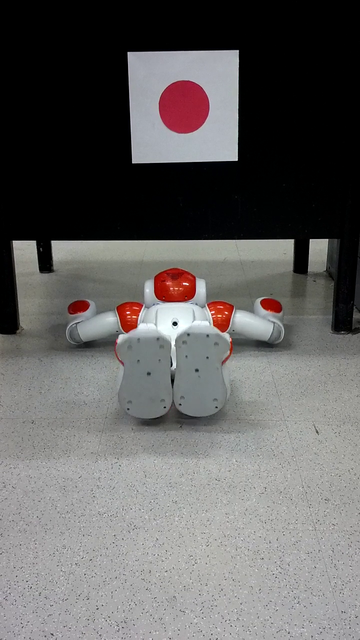
\includegraphics[width=0.2\textwidth]{crawl/walk_to/from/37s.png}
    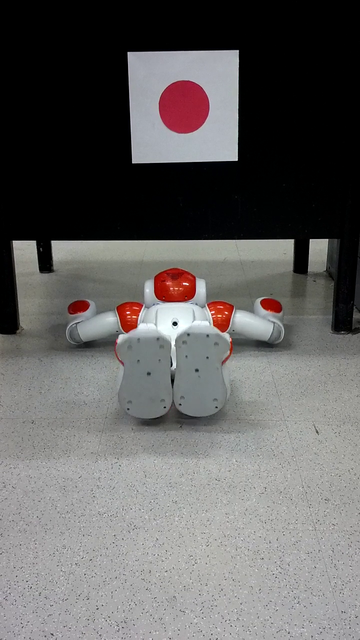
\includegraphics[width=0.2\textwidth]{crawl/walk_to/from/37s.png}
  }
  \caption{Figure showing arm joints and how they are a reflection.}
  \label{fig:nao_arm_joints_reflect1}
\end{figure}

Need diagram showing different postures for crawl results. 
\begin{figure}
  \centerline{
    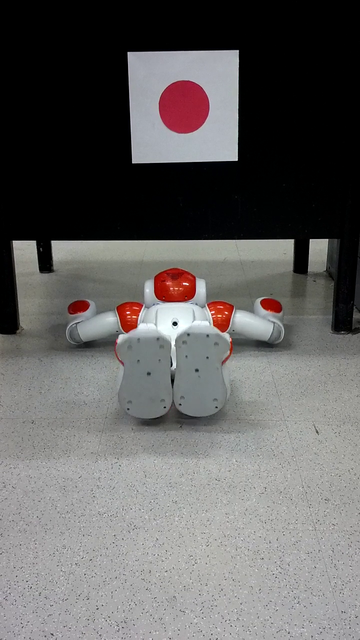
\includegraphics[width=0.2\textwidth]{crawl/walk_to/from/37s.png}
    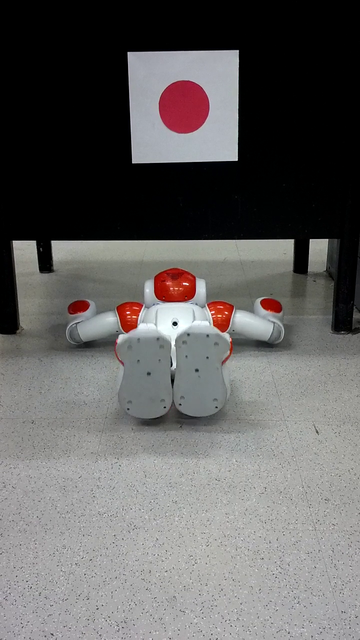
\includegraphics[width=0.2\textwidth]{crawl/walk_to/from/37s.png}
  }
  \caption{Figure showing postures.}
  \label{fig:nao_postures1}
\end{figure}

\subsection{Lidar Hardware}
Hokuyo is a Lidar. What's a Lidar? How does it work and what does it give you? 
{Diagrams explaining things}

Number of beams, angular resolution of beams, range of beams, resolution and accuracy.
Weight, power consumption, USB, update rate (sensor bandwidth).
Indoor only, not rated for outdoors.
[Diagram of Hokuyo.]

\subsection{Lidar Mount}
Design reqs: needed to rigidly attach to Nao for data transformation purposes, needed to see forward,
needed to be able to crawl with it, lightweight, Nao needed to be able to move his head while wearing it,
needed to be able to use the sonars (just in case).

Mounting it to the head seemed like it was going to be tough, so a vest was designed.
Straps and foam seemed like they'd hold well enough. In fact they hold so well I can lift Nao up by the mount.
[Show Solidworks design.]

\section{Software Framework}
So Nao comes with a much of good stuff. The API allows us to program in C++ or python and run locally or
remote. We can also test things quickly using Choreographe. Because it's linux we can also easily
run other non-aldebaran programs in python or using g++ complier.
The lidar runs on a python server, allowing the ground station and the Nao to easily see/use the data since
everything is over WiFi and the sockets don't care. How does this work?
How to log into Nao. Choreographe, remote run, and ssh for local run.

\subsection{NaoQi API and qibuild}
qibuild is what allows us to use the libraries remotely or locally without thinking. It's based on CMake
so you can add new libraries in just as you would with CMake on Linux.

The API is really a lot. You can command things on the joint level, nav level, pose level,
set velocities or positions, get orientation, distances, and joint angles or currents.
Everything is done with proxies.

% \subsection{Custom Library Framework}
\subsection{User Operation}
How do you start Nao, start Lidar? Log in to robot? Start program. Load program.
Start algorithms, stop them.
			
% \begin{table}[h!]
% 	\centering
% 	\begin{tabularx}{\textwidth}{|C{0.1}|C{0.4}||C{0.25}|C{0.25}|} 
% 		\hline
% 		\textbf{Net} 	&	\textbf{Device} 		&	\textbf{$V_{op}, V$}	&	\textbf{$I_{nom}, A$}	\\	\hline\hline
% 		1				&	AutoPilot (RM48, TM4C) 	& 	12.0					&	0.40	 				\\	\hline
% 		1				&	XBEE Radio 				&	3.3						&	0.25					\\ 	\hline
% 		1				&	ODROID-XU 				&	5.0						&	2.0						\\ 	\hline
% 		1				&	Logitech-9000			&	5.0						&	0.1						\\ 	\hline
% 		1				&	Hokuyo-URG				&	5.0						&	0.5 					\\	\hline
% 		2				&	AX12a Servos (x16)		&	12.0 					&	9.6	($~$0.6 ea.)		\\	\hline
% 	\end{tabularx} 
% 	\begin{tabularx}{\textwidth}{|C{0.5}|C{0.5}|} 
% 		\hline
% 		\textbf{Total Power Consumption} 		& 	137.8250 W \\\hline
% 		\textbf{Worst-Case Power Consumption}  	& 	$\approx$200.000 W \\\hline
% 	\end{tabularx} 
% 	\caption{Power consumption summary by device (for single-camera configuration).}
% 	\label{tab::power_summary}
% \end{table}


% \begin{table}[h!]
% 	\centering
% 	\begin{tabularx}{\textwidth}{|C{0.1}|C{0.4}||C{0.25}|C{0.25}|}
% 		\hline
% 		\textbf{Net} 		&	\textbf{Battery Pack}	&	\textbf{$V_{out}, V$}			&	\textbf{Rating, $A.hr$}	\\	\hline\hline
% 		1				&	3S LiPo Pack (x1)		& 	12.0						&	2.0	 					\\	\hline
% 		2				&	3S LiPo Pack (x3)		&	12.0						&	6.0						\\ 	\hline
% 	\end{tabularx}
% 	\begin{tabularx}{\textwidth}{|C{0.5}|C{0.5}|} 
% 		\hline
% 		\textbf{Average Runtime}  		& 	$\approx$41 minutes \\\hline
% 		\textbf{Worst-Case Runtime}  	& 	$\approx$28 minutes \\\hline
% 	\end{tabularx} 
% 	\caption{Battery power supply and estimated runtime summary.}
% 	\label{tab::runtime_summary}
% \end{table}